\documentclass{paper}
\usepackage{amsmath}
\usepackage{graphicx}
\usepackage{biblatex}
\addbibresource{ref.bib}

\title{Light-by-Light Scattering: Description \& Applications}
\author{Alfaifi, Ammar \and Al-Ali, Muhammad}
\date{\today}

\begin{document}

\maketitle

\begin{abstract}
	Light-light scattering, also known as photon-photon scattering, is a quantum electrodynamic (QED) phenomenon in which two photons interact and scatter off each other. In this paper, we discuss the theory of light-light scattering and present the Feynman diagrams for the process. We also discuss the implications of light-light scattering and its experimental verification.
\end{abstract}

\section{Introduction}

Light-light scattering, also known as photon-photon scattering, is a fundamental quantum electrodynamic (QED) process in which two photons interact and scatter off each other. The phenomenon was first predicted by Einstein in 1917~\cite{einstein}, who showed that photons have momentum and can exert a force on each other. However, it was not until the development of quantum field theory in the 1950s that a complete theory of light-light scattering was developed.

Light-light scattering is a purely quantum mechanical process and cannot be explained using classical physics. It is a rare phenomenon, as the probability of two photons interacting is very small. However, the process has important implications for the study of the fundamental nature of light and its interactions with matter.

In this paper, we discuss the theory of light-light scattering and present the Feynman diagrams for the process. We also discuss the implications of light-light scattering and its experimental verification.

\section{Theory of Light-Light Scattering}

The theory of light-by-light scattering was first proposed by physicist Richard Feynman in 1948. Feynman used a mathematical technique called Feynman diagrams to represent the interaction between particles. In a Feynman diagram, photons are represented by lines, and their interactions are represented by vertices where the lines meet.

Feynman diagrams show that light-by-light scattering is a very rare event because photons do not have any electric charge, and therefore, do not experience electromagnetic force. This means that photons do not interact with each other through the exchange of virtual particles such as gluons or W/Z bosons.

However, photons can still interact with each other through weak force, which is one of the four fundamental forces of nature. The weak force is responsible for the radioactive decay of atoms, but it is much weaker than the electromagnetic force. This is why light-by-light scattering is a very rare phenomenon.

In 2015, a team of scientists at the Large Hadron Collider (LHC) at CERN observed light-by-light scattering for the first time. The team used the LHC to collide two high-energy photons, which resulted in the scattering of the photons. This observation confirmed the theoretical predictions of light-by-light scattering and provided new insights into the fundamental nature of light.

Light-by-light scattering has many potential applications in the fields of physics, astronomy, and engineering. For example, it could be used to study the properties of dark matter and the structure of the universe. It could also be used to develop new technologies such as laser-based particle accelerators and high-precision sensors.

The theory of light-light scattering is based on quantum electrodynamics (QED), which is the quantum mechanical theory of the electromagnetic field and its interactions with charged particles. In QED, photons are treated as particles that can interact with each other through the exchange of virtual particles such as electron-positron pairs.

\begin{figure}[h]
	\centering
	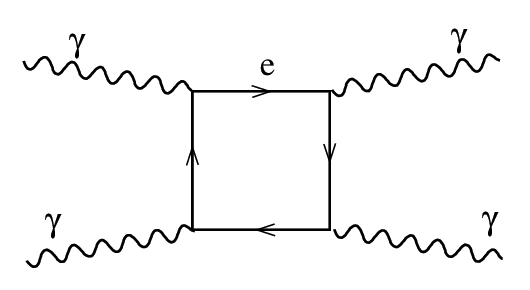
\includegraphics[width=0.5\linewidth]{figures/Feynman-diagram.png}
	\caption{Feynman diagrams for light-light scattering.}
	\label{fig:light-light-scattering-feynman}
\end{figure}
The Feynman diagrams for light-light scattering are shown in Figure~\ref{fig:light-light-scattering-feynman}. The process can be thought of as the interaction of two photons, labelled as 1 and 2, which scatter off each other and produce two outgoing photons, labelled as 3 and 4. The process is mediated by the exchange of a virtual electron-positron pair, which is created and annihilated in the process.


The probability of light-light scattering can be calculated using the Feynman diagrams and the rules of quantum electrodynamics. The result is a very small probability, which makes the phenomenon difficult to observe experimentally.

\section{Implications and Experimental Verification}

The phenomenon of light-light scattering has important implications for the study of the fundamental nature of light and its interactions with matter. It is a fundamental QED process that cannot be explained using classical physics and provides evidence for the quantum nature of light.

Light-light scattering has also been used to test the validity of QED.
The predicted probability of the process has been verified experimentally to a high degree of precision, providing strong evidence for

\subsection{ATLAS Observation}

\begin{figure}[ht]
	\centering
	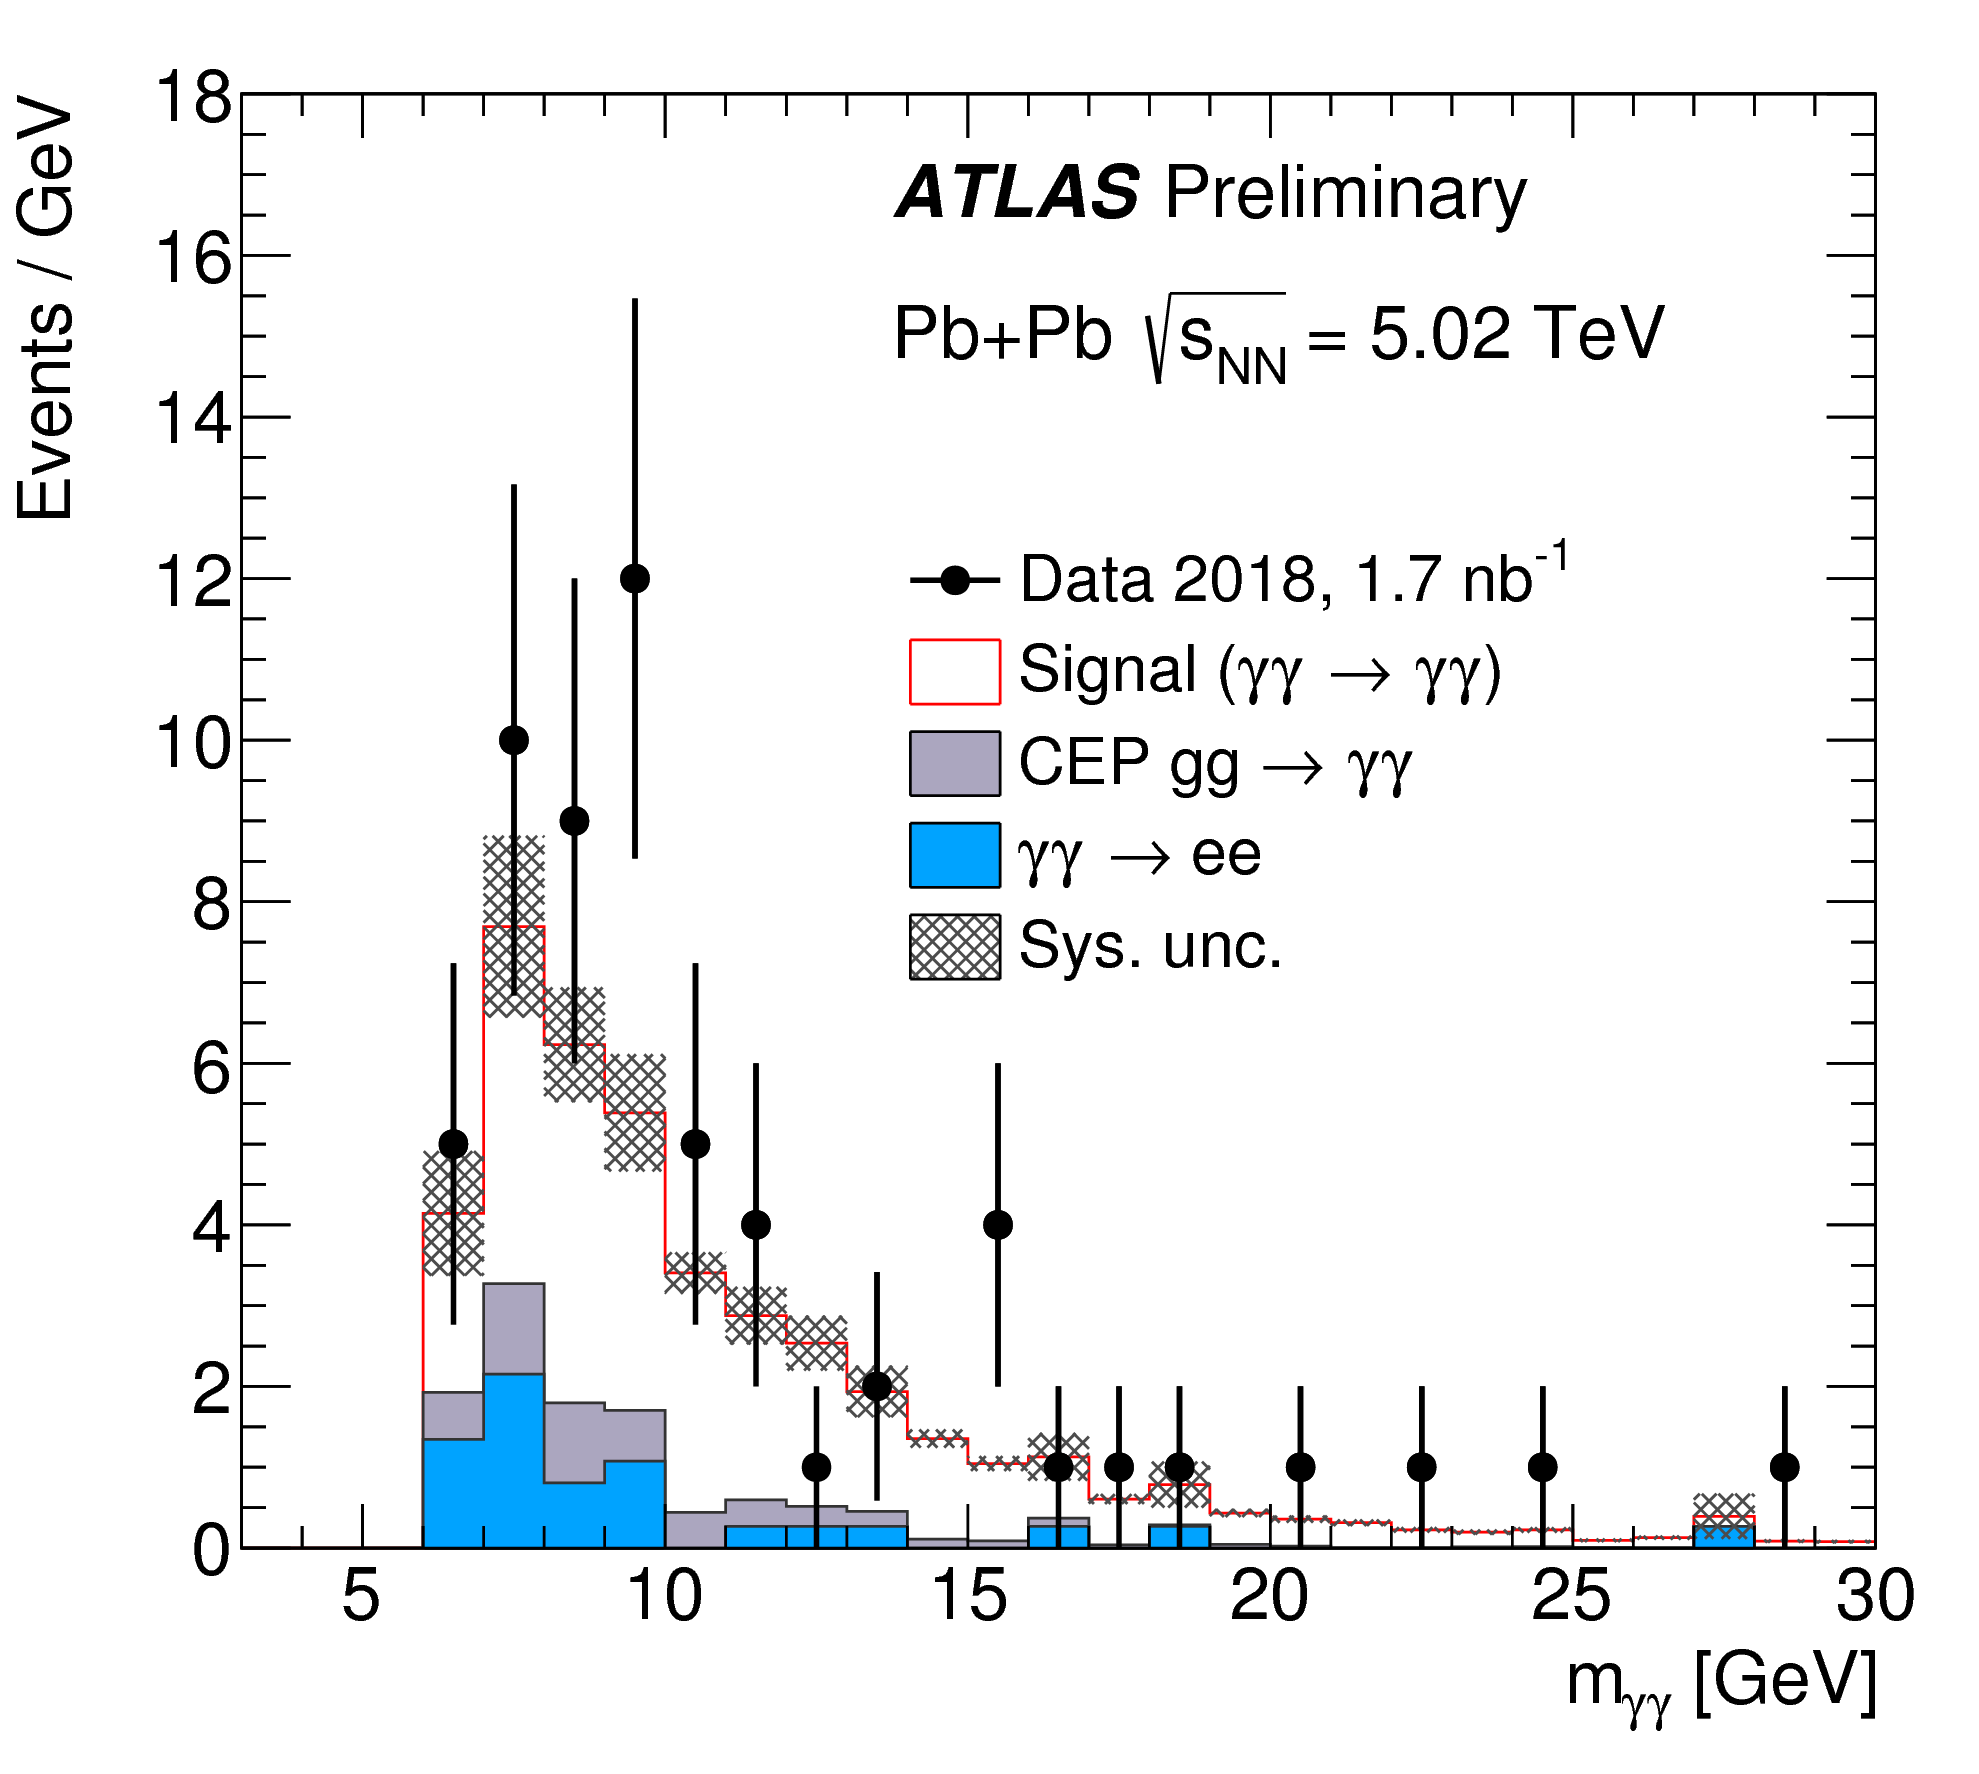
\includegraphics[width=0.5\linewidth]{figures/LbyL-fig2.png}
	\caption{Invariant mass distribution of the measured final state photon pairs (markers), compared
		to the expected light-by-light scattering signal (red line) and expected background contributions
		(shaded areas). (Image: ATLAS Collaboration/CERN)}
	\label{fig:Atlas data}
\end{figure}
Light-by-light scattering is a very rare phenomenon in which two photons – particles of light – interact,
producing another pair of photons. This process was among the earliest predictions of quantum electrodynamics (QED),
the quantum theory of electromagnetism, and is forbidden by classical physics theories (such as
Maxwell's theory of electrodynamics).


\begin{figure}[ht]
	\centering
	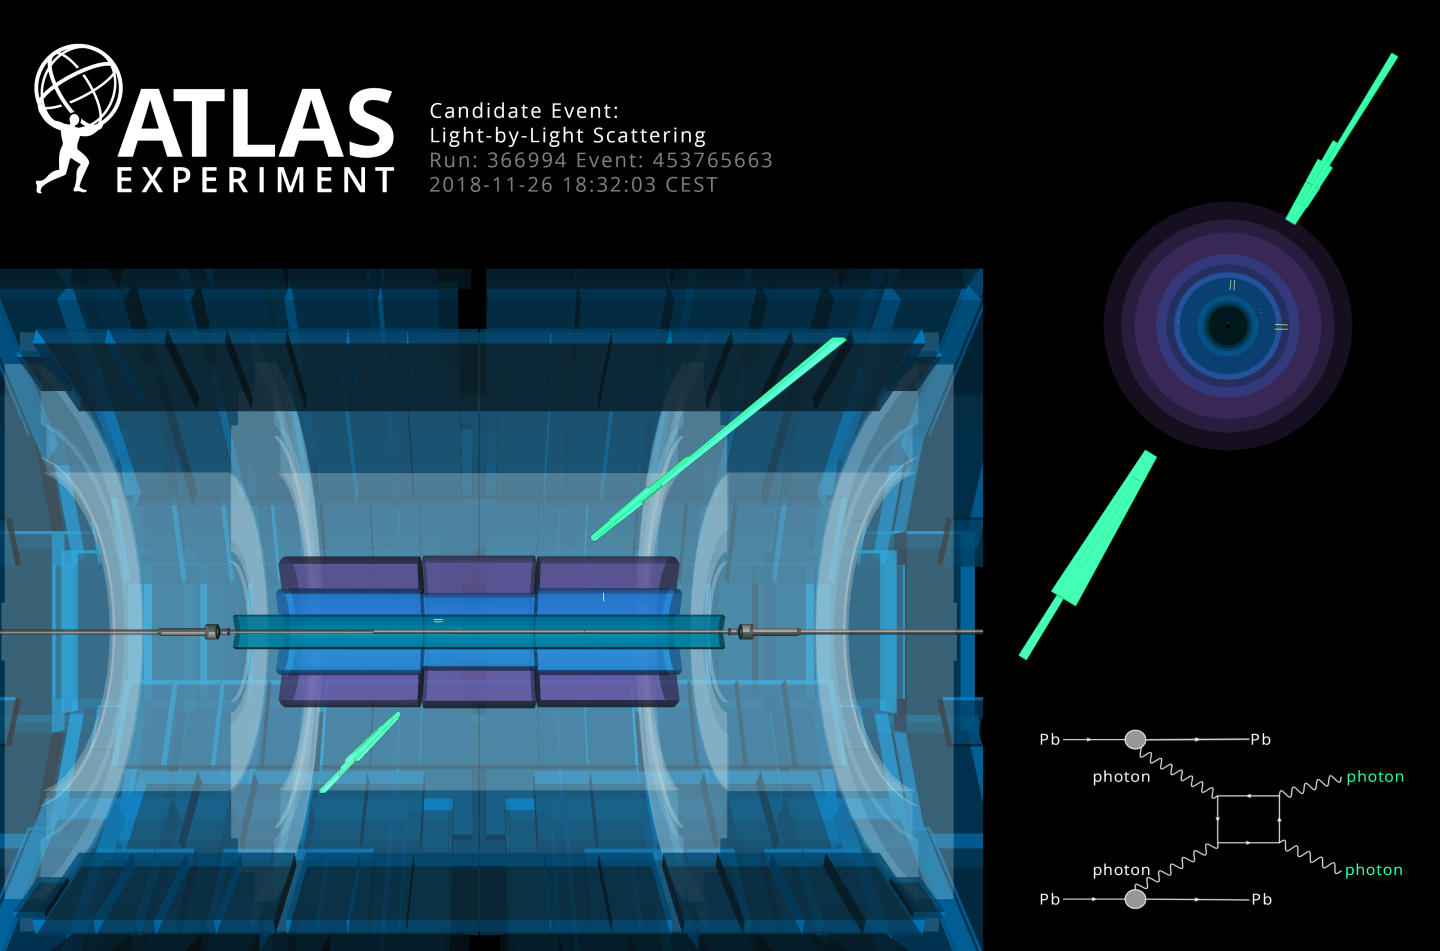
\includegraphics[width=0.5\linewidth]{figures/EventDisplay_LbyL.png}
	\caption{ATLAS event display shows the energy deposits of two photons in the electromagnetic
		calorimeter (green) on opposite sides and no other activity in the detector, which is the clear signature
		of light-by-light scattering. The Feynman diagram of this process is shown in the lower right corner.
		(Image: ATLAS Collaboration/CERN)}
	\label{fig:Atlas_event}
\end{figure}
Direct evidence for light-by-light scattering at high energy had proven elusive for decades until the Large Hadron
Collider (LHC) began its second data-taking period (Run 2). Collisions of lead ions in the LHC
provide a uniquely clean environment to study light-by-light scattering. Bunches of lead ions that are accelerated to
very high energy are surrounded by an enormous flux of photons. Indeed, the coherent action from the large number of
82 protons in a lead atom with all the electrons stripped off (as is the case for the lead ions in the LHC)
give rise to an electromagnetic field of up to 1025 Volt per metre. When two lead ions pass close by each
other at the centre of the ATLAS detector, but at a distance greater than twice the lead ion radius, those
photons can still interact and scatter off one another without any further interaction between the lead ions, as the reach of
the (much stronger) strong force is bound to the radius of a single proton. These interactions are
known as ultra-peripheral collisions.

`The ATLAS Collaboration has reported the observation of light-by-light scattering with a significance
beyond 8 standard deviations.`


In a result published in Nature Physics in 2017, the ATLAS Collaboration found thirteen candidate events for light-by-light scattering in lead-lead collision data recorded in 2015, for 2.6 events expected from background processes. The corresponding significance of this result was 4.4 standard deviations – making it the first direct evidence of high-energy light-by-light scattering.


\subsection{Light-by-Light Scattering at Low Energies}%

\begin{figure}[!th]
	\centering
	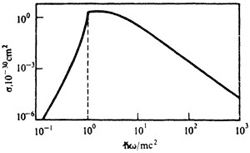
\includegraphics[width=0.5\linewidth]{figures/photon-photon-scattering.jpg}
	\caption{The cross-section for photon-photon scattering as a function of photon frequency (from Lifshitz et al. - 1982) }
	\label{fig:corss-secction}
\end{figure}

\begin{figure}[!th]
	\centering
	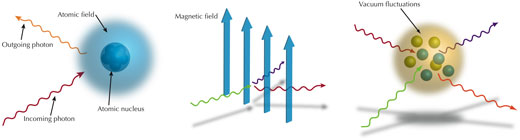
\includegraphics[width=\linewidth]{figures/photons.jpg}
	\caption{Three different types of interactions between photons. In the left picture, an incoming photon interacts with e.g. the strong external field from an atomic nucleus, resulting in an outgoing photon with new characteristics (Delbrück scattering); in the middle picture a single photon interacts with e.g. a strong external magnetic field as produce two low-frequency photons (photon splitting); finally, in the picture to the right two photons interacts directly via the quantum vacuum, producing two scattered photons. (Courtesy: Mattias Marklund)}
	\label{fig:photon-types}
\end{figure}
photon–photon scattering is a non-classical effect arising in quantum electrodynamics (QED) due to virtual electron–positron pairs in a vacuum. Under everyday circumstances, the effect is very weak, see Figure~\ref{fig:corss-secction}. However, under the right conditions, the interaction between photons and these virtual pairs will result in what is known as photon–photon collisions. Close relatives to this effect are Delbrück scattering and photon splitting, see Figure~\ref{fig:photon-types}. Formulated as an effective field theory, using the Heisenberg–Euler Lagrangian (Heisenberg \& Euler (1936); Schwinger (1951)), such scattering results in nonlinear corrections to Maxwell’s vacuum equations, similar in form to what is known as Kerr nonlinearities in nonlinear optics.
The effective self-interaction term in Maxwell’s equations is small (proportional to the fine structure constant squared), which means that the field strengths need to reach appreciable values until such e/Ndffects become pronounced (Marklund \& Shukla (2006); Mourou et al. (2006)). However, the smallness of the photon-photon scattering cross section has been argued to be a possible window to new physics (Anoniadis (1998); Arkani-Hamed et al. (1998); Cheung (1999); Davoudiasl (1999)), such as weak scale quantum gravity. Physical implications, as well as possible detection techniques, of the effects of photon–photon scattering have attracted interest since the 1930s (for surveys, see Refs. Marklund \& Shukla (2006) and Mourou et al. (2006) and references therein), and the topic is hotter than ever.

\subsection{Positron Production in Multiphoton Light-by-Light Scattering}%
\label{subsec:positron}

\label{subsec:light-light-low-energy}
A signal of 106±14 positrons above the background has been observed in collisions of a low-emittance 46.6 GeV electron beam with terawatt pulses from a Nd:glass laser at 527 nm wavelength in an experiment at the Final Focus Test Beam at SLAC. The positrons are interpreted as arising from a two-step process in which laser photons are backscattered to GeV energies by the electron beam followed by a collision between the high-energy photon and several laser photons to produce an electron-positron pair. These results are the first laboratory evidence for inelastic light-by-light scattering involving only real photons.\cite{physrevlett}



\section{Delbruck scattering}

Delbruck scattering to understand it first we need to understand a process called vacuum polarization.
Vacuum polarization is a random process by which a photon produces a pair of virtual fermion and anti-fermion and then annihilates repeatedly, the Feynman diagram of this process can be seen in the graph Figure~\ref{fig:corss-secction}.
Since this process involves charged particles (electron and anti-electron) this pair will create a virtual dipole and then would interact with other charged particles especially if the process occurred in nuclei. As a consequence of these interactions on the nucleus, the virtual electron will be attracted, and the virtual positron will be repelled creating a dipole that can cause shielding and reduce the charge if you were to observe from far enough.

\begin{figure}[!th]
	\centering
	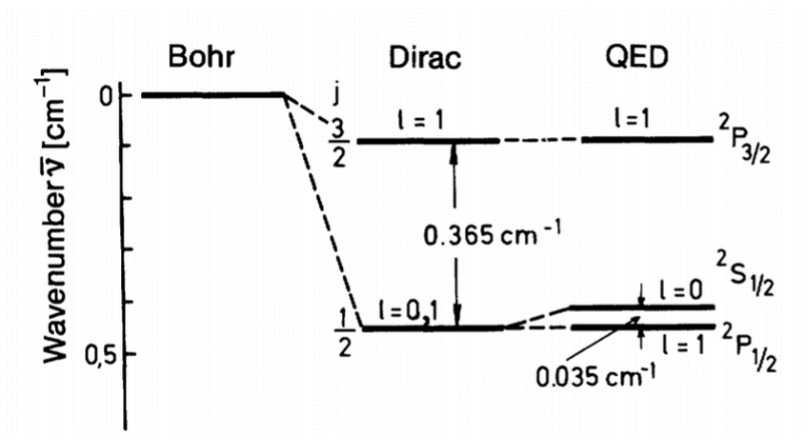
\includegraphics[width=0.5\linewidth]{figures/lamb-shift.png}
	\caption{the lamb shift compared to the prediction of Bohr and Dirac}
	\label{fig:lamb-shift}
\end{figure}
This shielding due to the vacuum polarization results in a deviation of the experimental Landé g-factor of the electron from the theoretical value and a difference in energy between two energy levels that was later called the “Lamb shift” Figure~\ref{fig:lamb-shift}, which contradicts the prediction of the Dirac equation. These theoretical deviations were calculated by the genius Hans Bethe, and what is funny is that he did the calculation on his return train ride when he was returning to Cornell after attending a select workshop in the summer of 1947 in Shelter Island.
Overall, Vacuum polarization was first discussed in papers by Paul Dirac and Werner Heisenberg in 1934, and the effects of it were calculated to first order in the coupling constant by Robert Serber and Edwin Uehling in 1935. But the effect of vacuum polarization of the electron and anti-electron was first observed in the 1940s, and for the quark and anti-quark, it was in the early 1970s.
Due to this phenomenon, the notion of vacuum changed, this is because the vacuum is not empty anymore but will have some fluctuation and the presence of this virtual particle will disturb the electromagnetic field, however, the fluctuation and the presence of these charged particles will follow the energy-time Heisenberg uncertainty principle so that they will annihilate quickly.
To sum up, vacuum polarization is the virtual fermion-antifermion produced from a vacuum-polarized disturbing electromagnetic field.

\begin{figure}[!th]
	\centering
	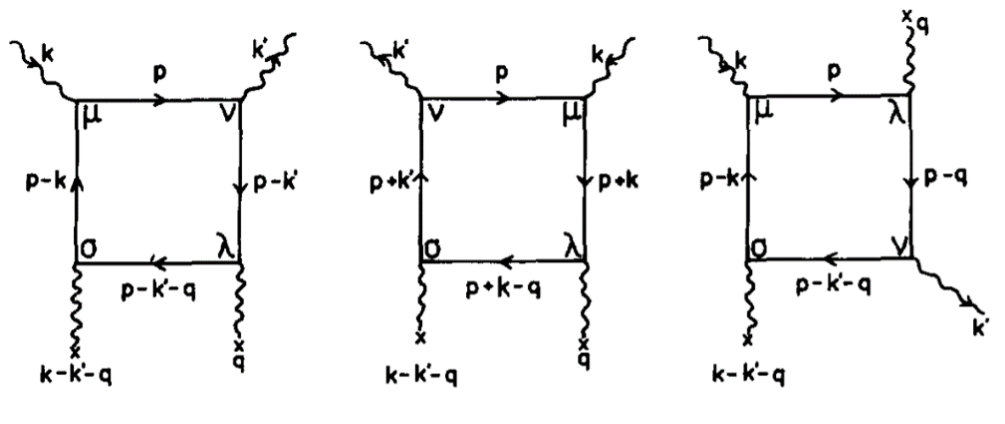
\includegraphics[width=0.5\linewidth]{figures/fyenman-diagram-Delbruck.png}
	\caption{Feynman diagrams for Delbruck scattering to lowest order, where x denotes Columb fields.}
	\label{fig:Feynman-Delbruck}
\end{figure}
Now, Delbruck scattering is the elastic scattering of photons in an electromagnetic field of nuclei (mostly heavy nuclei) as a consequence of the vacuum polarization, in which the two-photon scatters via electron-positron pairs as in the vacuum polarization Figure~\ref{fig:Feynman-Delbruck}.
This scattering depends on the energy of the photons and the angle, for each case whether high energy and small angles or intermediate energy and moderately large angles or at low energies but in the whole angular range, we will not go deep into the mathematics of each case since it’s extremely advanced, but the theoretical part is approached by some method called quasi-classical for the description of quantum electrodynamical processes in the Coulomb field at high energies.
Delbruck scattering is considered one of the nonlinear processes in quantum electrodynamics, along with photon splitting (in which a highly energetic photon turns in the electric field of an atom into two photons sharing its energy, and the observation of photon splitting is extremely hard) such that the interaction between the electromagnetic fields is not linear due to the polarizability of the vacuum, but what makes it the most interesting nonlinear processes that it can be precisely tested by experiment, also that it is an extremely interesting and successful experimental tool in nuclear physics.

It was first theoretically discovered in 1933 by Max Delbrück to account for the differences between what was observed in a Compton scattering experiment on heavier atoms (done by Meitner and Kösters) and what was predicted. Then it was confirmed 20 years later by Hans Bethe who named it “Delbrück scattering”. It was observed for the first time at DESY in 1973 for high-energy and small-angle photon scattering.

The cross-section of this process will have $Z_\alpha$ as parameters or $Z|e|$ after setting $\hbar=c=1$, and since this specific photon-photon scattering contain external fields mediating the interaction between photons, the cross-section will be larger than for pure photon-photon scattering.

\section{Breit–Wheeler process}

\begin{figure}[!th]
	\centering
	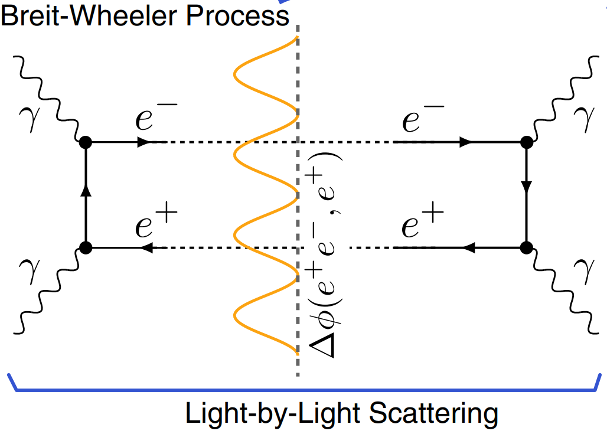
\includegraphics[width=0.5\linewidth]{figures/Breit-Wheeler.png}
	\caption{Feynman diagram of Breit–Wheeler pair process and the photon-photon scattering.}
	\label{fig:Feynman-diagram-of-Breit–Wheeler}
\end{figure}

\begin{figure}[!th]
	\centering
	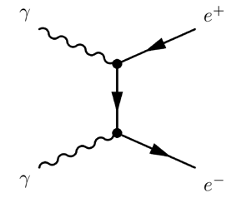
\includegraphics[width=0.5\linewidth]{figures/Feynman-Breit.png}
	\caption{Feynman diagram of Breit–Wheeler pair production.}
	\label{fig:Breit–Wheeler-pair}
\end{figure}

This process is another photo-photon interaction, and it resembles photon-photon scattering in which they both are scattering of two photons in the initial state, see Figure~\ref{fig:Feynman-diagram-of-Breit–Wheeler}.
Breit–Wheeler process is the collision of two photons then producing electron-positron pair see Figure~\ref{fig:Breit–Wheeler-pair}, it defined as
 $\gamma + \gamma' \rightarrow e^+ + e^-$, it was predicted first by Gregory Breit and John Wheeler in 1934 from the work of Dirac.
The energies of the photons must reach the threshold of the rest mass of the electron-positron pair, since the threshold for the electron-positron is much smaller than muon-antimuon, tau-antitau, quark-antiquark, it’s more likely to happen, however, the possibility of such process is very small in general.
The pair production is nearly impossible to occur just between two photons generated randomly, this triggers the idea of using two ionized gold atoms to create the highly energetic photons which will have larger cross-sections, using this idea the pair production was directly observed at “Relativistic Heavy Ion Collider” in 2021.
As the type of photons pair differ the process also will be different and each can be identified very easily in a collider, for example, the virtual-virtual photon collision is different from the virtual-real photon collision. The Breit–Wheeler is from the type of real-real photon collision it occurs at large angles. Also, there is another similar process in which a photon interacts with a laser field known as the multiphoton Breit–Wheeler process or nonlinear Breit–Wheeler.
It is strong evidence of Einstein’s equation $E=mc^2$ as it shows the conversion from energy to matter.



\section{Conclusion}
With the help of advanced technologies such as the LHC and Feynman diagrams, we can continue to study and learn more about this elusive interaction.
Light by light scattering is a phenomenon in which two photons interact and produce a new photon. This process is extremely rare and difficult to observe, but it has important implications for our understanding of the universe.

One of the most significant applications of light-by-light scattering is in the study of the behaviour of particles at very high energies. By studying the scattering of photons, scientists can learn more about the properties of fundamental particles such as electrons and quarks. This knowledge can help us better understand the fundamental forces that govern the universe, such as electromagnetism and the strong and weak nuclear forces.

Additionally, light-by-light scattering can be used to study the properties of materials. By shining a laser at a material and analyzing the scattered light, scientists can determine the composition, structure, and other properties of the material. This can be useful for a variety of applications, including materials science and medical imaging.

In conclusion, light-by-light scattering is a fascinating phenomenon that has important applications in a variety of fields. By studying the scattering of photons, we can learn more about the fundamental forces that govern the universe and the properties of materials. This knowledge can help us advance our understanding of the world around us and develop new technologies.

\newpage
\nocite{*}
\printbibliography

\end{document}
